\chapter{Results and Discussion}

\section{Model Parameters}

Using the $70\%$ training set, $15\%$ validation set, and $15\%$ testing set, the hyperparameters chosen for each learning model is shown in \cref{tab:hyperparam}.

\begin{table}[h]
	\centering
	\caption{Final hyperparameters for learning models}
	\label{tab:hyperparam}
	\begin{tabular}{@{}ll}
		\toprule
		Model                & Parameters                                                                                    \\ \midrule
		Ridge Regression     & $\lambda=10$                                                                                  \\ \midrule
		Huber Regression     & $\epsilon = 1.0$                                                                              \\
		                     & $\alpha=0.001$                                                                                \\
		                     & ($\epsilon$ and $\alpha$ are specific to the Scikit-learn implementation \cite{scikit-learn}) \\\midrule
		\acs{MLP}            & Size of first hidden layer: $200$                                                             \\
		                     & Size of second hidden layer: $150$                                                            \\ \midrule
		\acs{CNN}            & $L_2$ Regularization: $\lambda=0.8$                                                           \\
		                     & Convolution layers depth: $(128, 256)$                                                        \\
		                     & Fully connected layers size: $(512, 256)$                                                     \\ \midrule
		\acs{CNN}+\acs{LSTM} & $L_2$ Regularization: $\lambda=0.0001$                                                             \\
		                     & \acs{LSTM} hidden state size: 4096                                                            \\
		                     & Convolution block size for three convolution blocks: $(64, 128, 256)$                         \\ \bottomrule
	\end{tabular}
\end{table}

\section{Cross Validation Results}


\begin{figure}[p]
\begin{minipage}{\textwidth}
	\centering
	\begin{subfigure}[b]{\textwidth}
		\centering
		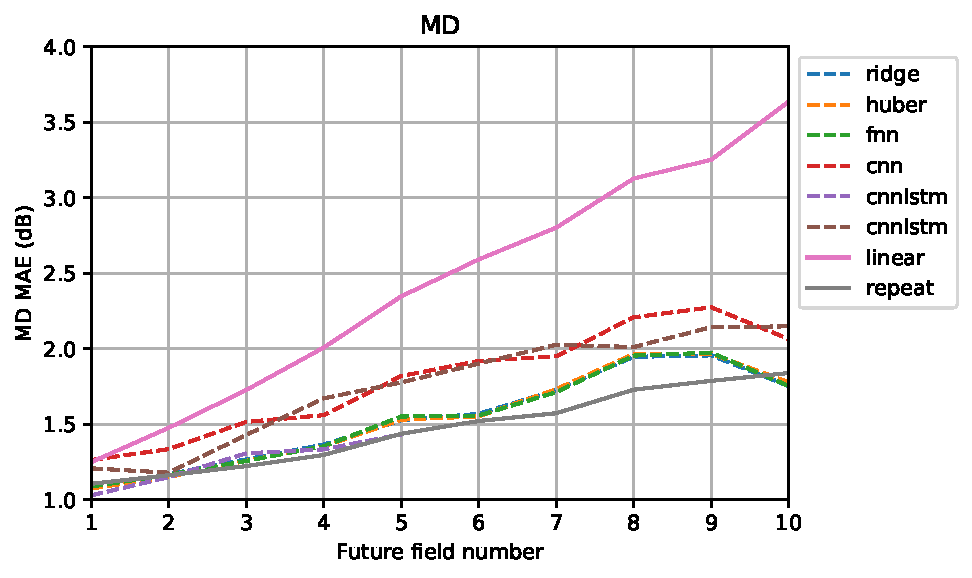
\includegraphics[width=0.8\textwidth]{ml_md.pdf}
		\caption{}
	\end{subfigure}
	\hfill
	\begin{subfigure}[b]{\textwidth}
		\centering
		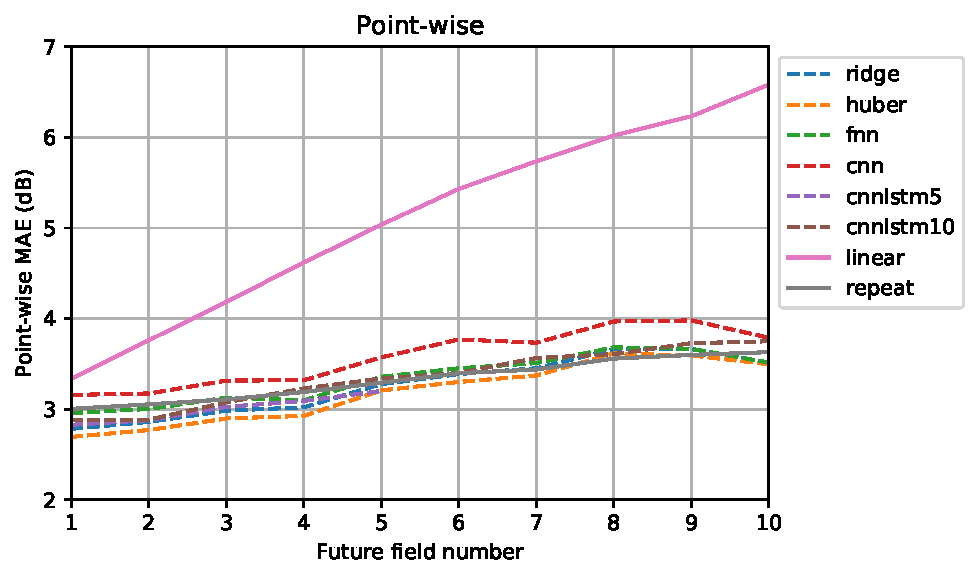
\includegraphics[width=0.8\textwidth]{ml_vf.pdf}
		\caption{}
	\end{subfigure}
	\caption[\acs{MD} and point-wise field prediction results for learning algorithms]{\acs{MD} and point-wise field prediction results for learning algorithms with 3 inputs, compared to the linear extrapolator and repeating the last observed value ``repreat''. There is no significant difference between the learning methods, and due to the dataset containing mostly stable patients, there is no significant difference between the learning methods and ``repeat''. However, all methods performed better than the linear extrapolation methods. \footnote{In an earlier version of this figure, it was shown that the CNN+LSTM model performed slightly better than other learning methods. This has been corrected in this latest batch of experiments.}}
	\label{fig:ml_fig}
\end{minipage}
\end{figure}

\begin{table}[t]
	\centering
	\caption{Learning algorithm performance for the 5-th and 10-th prediction}
	(25\%/50\%/75\% are the 25-th percentile/median/75-th percentile respectively)
	\label{tab:ml_tab}
	
	\hspace*{-1.5cm}
	\begin{tabular}{@{}llllllllll@{}}
		\toprule
		Prediction &      &   \multicolumn{6}{c}{Learning Algorithm} &  \multicolumn{2}{c}{Extrapolation}  \\
		\cmidrule(lr){3-8} \cmidrule(lr){9-10}
		\acs{MAE} (dB) &      & Ridge & Huber & \acs{MLP}  & \acs{CNN}  & CNN+LSTM5 & CNN+LSTM10 & Linear & Repeat \\ \midrule
		& mean & 1.53  & 1.53  & 1.55 & 1.82 & 1.43     & 1.78      & 2.35   & 1.44   \\
		MD, & std  & 1.7   & 1.73  & 1.76 & 1.83 & 1.44     & 1.63      & 2.75   & 1.59   \\
		5-th& 25\% & 0.45  & 0.45  & 0.44 & 0.59 & 0.49     & 0.59      & 0.64   & 0.43   \\
		& 50\% & 1.05  & 1.02  & 1.04 & 1.3  & 1.03     & 1.44      & 1.41   & 0.99   \\
		& 75\% & 1.93  & 1.93  & 1.97 & 2.5  & 1.93     & 2.3       & 2.95   & 1.85   \\
		\midrule
		& mean & 1.75  & 1.78  & 1.75 & 2.06 &          & 2.15      & 3.64   & 1.84   \\
		MD, & std  & 1.75  & 1.76  & 1.78 & 2.01 &          & 2.16      & 4.28   & 2.17   \\
		10-th & 25\% & 0.57  & 0.6   & 0.57 & 0.64 &          & 0.65      & 0.81   & 0.51   \\
		& 50\% & 1.27  & 1.27  & 1.23 & 1.45 &          & 1.47      & 1.91   & 1.18   \\
		& 75\% & 2.32  & 2.29  & 2.24 & 2.8  &          & 2.79      & 4.94   & 2.3    \\
		\midrule
		& mean & 3.28  & 3.21  & 3.36 & 3.57 & 3.2      & 3.34      & 5.04   & 3.29   \\
		Point-wise, & std  & 3.55  & 3.63  & 3.85 & 4.08 & 3.69     & 3.87      & 5.85   & 4.18   \\
		5-th& 25\% & 0.95  & 0.89  & 0.88 & 0.94 & 1        & 1         & 1      & 1      \\
		& 50\% & 2.14  & 2.02  & 2.04 & 2.21 & 1.91     & 1.94      & 3      & 2      \\
		& 75\% & 4.25  & 4.1   & 4.27 & 4.53 & 4        & 4.1       & 7      & 4      \\
		\midrule
		& mean & 3.51  & 3.5   & 3.51 & 3.79 &          & 3.75      & 6.58   & 3.63   \\
		Point-wise, & std  & 3.58  & 3.74  & 3.86 & 4.16 &          & 4.33      & 7.39   & 4.6    \\
		10-th& 25\% & 1.11  & 1.05  & 1    & 1.03 &          & 1         & 1      & 1      \\
		& 50\% & 2.42  & 2.34  & 2.24 & 2.41 &          & 2.21      & 4      & 2      \\
		& 75\% & 4.61  & 4.54  & 4.54 & 4.94 &          & 4.64      & 10     & 5      \\ \bottomrule
	\end{tabular}
\end{table}

5-fold cross validation is performed on the learning models with hyperparameters listed in \cref{tab:hyperparam}. The same cross-validation set is used for ridge regression, Huber regression, \ac{MLP}, and \ac{CNN}. A different sequence is used for the \acs{CNN}+\acs{LSTM} model due to the recurrent structure of the \ac{LSTM} module; sequences extending to 5 and 10 fields into the future are investigated for \acs{CNN}+\acs{LSTM}. These results are compared to the linear extrapolation method and the repeat-last-value (``repreat'') method, which were described in \cref{sec:extrapresult}. A detailed comparison of the performance of different methods at predicting 5 and 10 fields in the future is tabulated in \cref{tab:ml_tab}.

Using the Rotterdam dataset, there is no significant difference between the learning algorithms evaluated for both the \ac{MD} prediction task \ac{MAE} and the point-wise whole field task \ac{MAE}. Furthermore, there is no significant difference between the learning and repeat method for both tasks. The linear extrapolation method performed much worse than all other methods in terms of mean, median, and 75-th percentile error, but the 25-th percentile error is similar. 

Within each method, the error increases as one extends the prediction further into the future. In addition, the \ac{MD} prediction \ac{MAE} is in general approximately one half that of the point-wise prediction \ac{MAE}. These observations are in agreement with expectation. 

\section{Discussion}

\begin{table}[h]
\centering
\caption{Glaucoma progression rates and study dataset statistics of \acs{EMGT}, \acs{CGS}, and Rotterdam}
\label{tab:glaucprogress}
\begin{tabular}{@{}llll@{}}
	\toprule
	                               &                      \multicolumn{3}{c}{Study}                       \\
	\cmidrule{2-4}                 & \acs{EMGT} \cite{Heijl2009} & \acs{CGS} \cite{Group2010} & Rotterdam \\ \midrule
	\textit{Progression (db/year)} &                             &                            &           \\
	mean                           & -1.08                       & -0.54                      & -0.10     \\
	std                            & 2.07                        & 1.10                       & 0.46      \\
	25\%                           &                             & -0.76                      & -0.21     \\
	50\%                           & -0.40                       & -0.35                      & -0.04     \\
	75\%                           &                             & -0.12                      & 0.12      \\
	interquartile range            & 1.05                        & 0.64                       & 0.33      \\ \midrule
	\textit{Age (years)}           &                             &                            &           \\
	N ($<68$)                      & 53 (45\%)                    &                            & 108 (78\%)          \\
	N ($\geq68$)                   & 65 (55\%)                    &                            & 31 (22\%)          \\
	mean                           & 68.0                        &                            & 59.7          \\
	std                            & 5.1                         &                            & 10.3         \\
	25\%                           &                             & 63.5                       & 52.7         \\
	50\%                           & 68                          & 68.2                       & 61.3          \\
	75\%                           &                             & 75.1                       & 67.6          \\ \bottomrule
\end{tabular}
\end{table}

The distribution of glaucoma progression rates, expressed in dB/year, is known to be asymmetric with a long tail for highly negative progression rates---some but only limited patients show very rapid progression, but most are reasonably stable as mild progressors. \cite{Anderson2015} In the \ac{EMGT}, Heijl et al. found that the rate of visual field loss in their study sample is: mean $-1.08$ dB/year, median $-0.40$ dB/year, interquartile range $1.05$ dB/year. \cite{Heijl2009} Chauhan et al. reported in the \ac{CGS}: mean $-0.54$ dB/year, median $-0.35$ dB/year, interquartile range $0.64$ dB/year. \cite{Group2010} Both studies reported that elder patients are more likely to progress faster. Heijl et al. reported that exfoliation glaucoma progresses much faster than non-exfoliation glaucoma patients. 

For the Rotterdam dataset used in this work, the rate of change values are: mean $-0.10$ dB/year, median $-0.04$, interquartile range $0.33$. Relevant statistics comparison is shown in \cref{tab:glaucprogress}. Overall, the progression rate is slower (less negative) than the two major studies. The patient population is younger. Furthermore, pseudo-exfoliation glaucoma was not included in the Rotterdam dataset. This causes the major limitation of current work in terms of algorithm training and testing, because most patients in the dataset are not demonstrating progression. As a result, the ``repeat'' prediction has the same effectiveness as learning methods. 

It is also found that the linear extrapolation methods, which is the current clinically adopted method, performed much worse than the other methods. If this suggests limitations in the linear extrapolation method for accurate prediction and slope estimation requires further investigation. The exponential model, despite its potential physiological interpretation, performs even worse than linear extrapolation. The fact that all learning methods managed to perform better suggests there is an application for such algorithms in the glaucoma prediction task. 

\section{Future Work}

The next step in the project is to collect a glaucoma patient dataset from our own sources. Such a dataset should include more examples of glaucoma progression by including older patients, patients with exfoliation glaucoma, and a larger patient sample size. 

Most current study datasets also does not include any patients with history of surgical intervention. However, patients with surgical intervention are also likely ones with the most severe progression rate and require the most attention for a carefully-determined treatment decision. We propose to also collect some patients with significant interventions, along with other potentially important details such as their medication history, family history, ethnicity, specific diagnosis, angle closure, etc., all of which are known to affect the trajectory of glaucoma progression. We will also attempt to collect \ac{OCT} data from the patients who will be included in our study. The challenge then lies in designing an algorithm that can appropriately represent such a multi-variable dataset. 

Finally, another area of application of machine learning algorithm is glaucoma screening, specifically the classification of patients in a screening setting. The input to the algorithm will be one visual field produced from a screening setting, potentially with \ac{IOP} information which is also routinely examined, and the algorithm will label if the patient is healthy or a glaucoma suspect. The performance of such an algorithm will be primarily compared against using field indices, especially \ac{GHT} which is designed for a similar classification task. 

